\documentclass[12pt]{article}
\usepackage{amsmath, amsthm, amssymb}
\usepackage{hyperref}
\usepackage{verbatim}
\usepackage[top=1.0in, bottom=1.0in, left=1.0in, right=1.0in]{geometry}

\pagestyle{plain}

\usepackage{tkz-graph}
\usetikzlibrary{arrows}
\usetikzlibrary{shapes}
\usepackage[position=bottom]{subfig}
\usepackage{graphicx}


\usepackage{longtable}
\usepackage{array}

\usepackage{sectsty}
\allsectionsfont{\sffamily}

\setcounter{secnumdepth}{5}
\setcounter{tocdepth}{5}

\makeatletter
\newtheorem*{rep@theorem}{\rep@title}
\newcommand{\newreptheorem}[2]{
\newenvironment{rep#1}[1]{
 \def\rep@title{#2 \ref{##1}}
 \begin{rep@theorem}}
 {\end{rep@theorem}}}
\makeatother

\theoremstyle{plain}
\newtheorem{thm}{Theorem}[section]
\newreptheorem{thm}{Theorem}
\newtheorem{prop}[thm]{Proposition}
\newreptheorem{prop}{Proposition}
\newtheorem{lem}[thm]{Lemma}
\newreptheorem{lem}{Lemma}
\newtheorem{conjecture}[thm]{Conjecture}
\newreptheorem{conjecture}{Conjecture}
\newtheorem{cor}[thm]{Corollary}
\newreptheorem{cor}{Corollary}
\newtheorem{prob}[thm]{Problem}

\newtheorem*{SmallPotLemma}{Small Pot Lemma}
\newtheorem*{BK}{Borodin-Kostochka Conjecture}
\newtheorem*{BK2}{Borodin-Kostochka Conjecture (restated)}
\newtheorem*{Reed}{Reed's Conjecture}
\newtheorem*{ClassificationOfd0}{Classification of $d_0$-choosable graphs}


\theoremstyle{definition}
\newtheorem{defn}{Definition}
\theoremstyle{remark}
\newtheorem*{remark}{Remark}
\newtheorem*{problem}{Problem}
\newtheorem{example}{Example}
\newtheorem*{question}{Question}
\newtheorem*{observation}{Observation}

\newcommand{\fancy}[1]{\mathcal{#1}}
\newcommand{\C}[1]{\fancy{C}_{#1}}
\newcommand{\IN}{\mathbb{N}}
\newcommand{\IR}{\mathbb{R}}
\newcommand{\G}{\fancy{G}}
\newcommand{\CC}{\fancy{C}}
\newcommand{\D}{\fancy{D}}

\newcommand{\inj}{\hookrightarrow}
\newcommand{\surj}{\twoheadrightarrow}

\newcommand{\set}[1]{\left\{ #1 \right\}}
\newcommand{\setb}[3]{\left\{ #1 \in #2 \mid #3 \right\}}
\newcommand{\setbs}[2]{\left\{ #1 \mid #2 \right\}}
\newcommand{\card}[1]{\left|#1\right|}
\newcommand{\size}[1]{\left\Vert#1\right\Vert}
\newcommand{\ceil}[1]{\left\lceil#1\right\rceil}
\newcommand{\floor}[1]{\left\lfloor#1\right\rfloor}
\newcommand{\func}[3]{#1\colon #2 \rightarrow #3}
\newcommand{\funcinj}[3]{#1\colon #2 \inj #3}
\newcommand{\funcsurj}[3]{#1\colon #2 \surj #3}
\newcommand{\irange}[1]{\left[#1\right]}
\newcommand{\join}[2]{#1 \mbox{\hspace{2 pt}$\ast$\hspace{2 pt}} #2}
\newcommand{\djunion}[2]{#1 \mbox{\hspace{2 pt}$+$\hspace{2 pt}} #2}
\newcommand{\parens}[1]{\left( #1 \right)}
\newcommand{\brackets}[1]{\left[ #1 \right]}
\newcommand{\DefinedAs}{\mathrel{\mathop:}=}

\def\adj{\leftrightarrow}
\def\nonadj{\not\!\leftrightarrow}

\def\D{\fancy{D}}
\def\C{\fancy{C}}

\newcommand{\bigclique}[1]{\frac{2}{3}\Delta(#1) + 5}
\newcommand{\bigcliqueraw}{\frac{2}{3}\Delta + 5}
\newcommand{\cliqueparts}{\frac{2}{3}\Delta}


\title{Coloring from almost maximum degree sized palettes}
\author{Landon Rabern}
\date{\today}

\begin{document}
\maketitle

\section{Introduction}
My dissertation contains material on a bunch of topics all relating to graph coloring, but today I'm going to almost entirely restrict myself to talking about a conjecture of Borodin and Kostochka from 1977.  First, i need to define some terms.

Define, $\Delta(G)$, $K_t$, coloring.  PICTURES.

\begin{conjecture}
Every graph $G$ with $\Delta(G) \geq 9$ that doesn't contain $K_{\Delta(G)}$ is $(\Delta(G)-1)$-colorable.
\end{conjecture}

Talk, $K_\Delta$ is the obvious obstruction to $(\Delta-1)$-coloring.

The classical theorem of Brooks from 1941 says:

\begin{thm}[Brooks 1941]
Every graph $G$ with $\Delta(G) \geq 3$ that doesn't contain $K_{\Delta(G) + 1}$ is $\Delta(G)$-colorable.
\end{thm} 

The $\Delta \geq 9$ condition is necessary:

\begin{figure}[htb]
\centering
\subfloat[$\Delta=6$]{
{\parbox{5cm}{
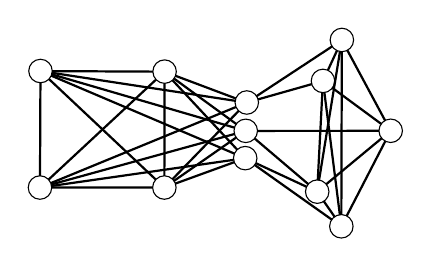
\begin{tikzpicture}[scale = 10]
\tikzstyle{VertexStyle}=[shape = circle, minimum size = 1pt, inner sep = 3pt,
draw]
\Vertex[x = 0.25085711479187, y = 0.92838092893362, L = \tiny {}]{v0}
\Vertex[x = 0.0932380929589272, y = 0.929142817854881, L = \tiny {}]{v1}
\Vertex[x = 0.250571489334106, y = 0.781142801046371, L = \tiny {}]{v2}
\Vertex[x = 0.092571459710598, y = 0.781142845749855, L = \tiny {}]{v3}
\Vertex[x = 0.355238050222397, y = 0.889142841100693, L = \tiny {}]{v4}
\Vertex[x = 0.353904783725739, y = 0.853142827749252, L = \tiny {}]{v5}
\Vertex[x = 0.353238135576248, y = 0.818476170301437, L = \tiny {}]{v6}
\Vertex[x = 0.476000010967255, y = 0.968571435660124, L = \tiny {}]{v7}
\Vertex[x = 0.537999987602234, y = 0.853238105773926, L = \tiny {}]{v8}
\Vertex[x = 0.444666564464569, y = 0.77590474486351, L = \tiny {}]{v9}
\Vertex[x = 0.475333333015442, y = 0.731904745101929, L = \tiny {}]{v10}
\Vertex[x = 0.451999962329865, y = 0.916571423411369, L = \tiny {}]{v11}
\Edge[](v0)(v1)
\Edge[](v2)(v1)
\Edge[](v3)(v1)
\Edge[](v0)(v3)
\Edge[](v2)(v3)
\Edge[](v2)(v0)
\Edge[](v4)(v2)
\Edge[](v5)(v2)
\Edge[](v6)(v2)
\Edge[](v4)(v0)
\Edge[](v5)(v0)
\Edge[](v6)(v0)
\Edge[](v4)(v1)
\Edge[](v5)(v1)
\Edge[](v6)(v1)
\Edge[](v4)(v3)
\Edge[](v5)(v3)
\Edge[](v6)(v3)
\Edge[](v8)(v7)
\Edge[](v9)(v7)
\Edge[](v10)(v7)
\Edge[](v11)(v7)
\Edge[](v9)(v8)
\Edge[](v10)(v8)
\Edge[](v11)(v8)
\Edge[](v10)(v9)
\Edge[](v11)(v9)
\Edge[](v11)(v10)
\Edge[](v4)(v7)
\Edge[](v4)(v11)
\Edge[](v6)(v9)
\Edge[](v6)(v10)
\Edge[](v5)(v8)
\Edge[](v5)(v9)
\end{tikzpicture}}}}\qquad\qquad
\subfloat[$\Delta=7$]{
{\parbox{5cm}{

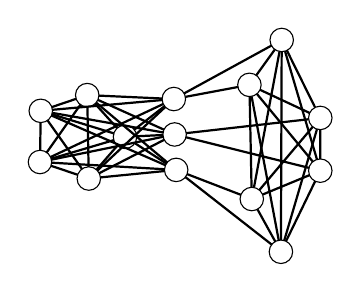
\begin{tikzpicture}[scale = 5]
\tikzstyle{VertexStyle}=[shape = circle, minimum size = 1pt, inner sep = 3pt,
draw]
\Vertex[x = 0.751999914646149, y = 0.724000096321106, L = \tiny {}]{v0}
\Vertex[x = 0.751999974250793, y = 0.590000092983246, L = \tiny {}]{v1}
\Vertex[x = 0.652000069618225, y = 0.38400000333786, L = \tiny {}]{v2}
\Vertex[x = 0.578000009059906, y = 0.51800012588501, L = \tiny {}]{v3}
\Vertex[x = 0.572000086307526, y = 0.808000028133392, L = \tiny {}]{v4}
\Vertex[x = 0.0419999808073044, y = 0.742000013589859, L = \tiny {}]{v5}
\Vertex[x = 0.0399999916553497, y = 0.612000048160553, L = \tiny {}]{v6}
\Vertex[x = 0.163999989628792, y = 0.569999992847443, L = \tiny {}]{v7}
\Vertex[x = 0.25600004196167, y = 0.676000028848648, L = \tiny {}]{v8}
\Vertex[x = 0.159999996423721, y = 0.782000005245209, L = \tiny {}]{v9}
\Vertex[x = 0.653999924659729, y = 0.921999998390675, L = \tiny {}]{v10}
\Vertex[x = 0.379999995231628, y = 0.771999999880791, L = \tiny {}]{v11}
\Vertex[x = 0.381999999284744, y = 0.682000011205673, L = \tiny {}]{v12}
\Vertex[x = 0.386000007390976, y = 0.592000007629395, L = \tiny {}]{v13}
\Edge[](v0)(v4)
\Edge[](v1)(v4)
\Edge[](v2)(v4)
\Edge[](v3)(v4)
\Edge[](v0)(v3)
\Edge[](v1)(v3)
\Edge[](v2)(v3)
\Edge[](v0)(v2)
\Edge[](v1)(v2)
\Edge[](v0)(v1)
\Edge[](v5)(v6)
\Edge[](v5)(v7)
\Edge[](v5)(v8)
\Edge[](v5)(v9)
\Edge[](v6)(v7)
\Edge[](v6)(v8)
\Edge[](v6)(v9)
\Edge[](v7)(v8)
\Edge[](v7)(v9)
\Edge[](v8)(v9)
\Edge[](v0)(v10)
\Edge[](v1)(v10)
\Edge[](v2)(v10)
\Edge[](v3)(v10)
\Edge[](v4)(v10)
\Edge[](v5)(v11)
\Edge[](v6)(v11)
\Edge[](v7)(v11)
\Edge[](v8)(v11)
\Edge[](v9)(v11)
\Edge[](v5)(v12)
\Edge[](v6)(v12)
\Edge[](v7)(v12)
\Edge[](v8)(v12)
\Edge[](v9)(v12)
\Edge[](v5)(v13)
\Edge[](v6)(v13)
\Edge[](v7)(v13)
\Edge[](v8)(v13)
\Edge[](v9)(v13)
\Edge[](v11)(v10)
\Edge[](v11)(v4)
\Edge[](v12)(v0)
\Edge[](v12)(v1)
\Edge[](v13)(v3)
\Edge[](v13)(v2)
\end{tikzpicture}}}}\qquad\qquad
\subfloat[$\Delta=7$~~~~~~~~~~~~~~~]{
{\parbox{5cm}{

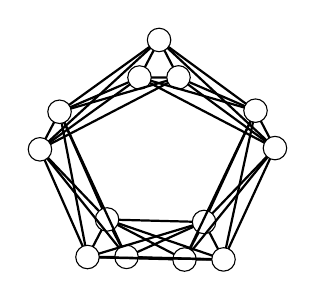
\begin{tikzpicture}[scale = 10]
\tikzstyle{VertexStyle}=[shape = circle, minimum size = 1pt, inner sep = 3pt,
draw]
\Vertex[x = 0.257401078939438, y = 0.729450404644012, L = \tiny {}]{v0}
\Vertex[x = 0.232565611600876, y = 0.681758105754852, L = \tiny {}]{v1}
\Vertex[x = 0.383801102638245, y = 0.820650428533554, L = \tiny {}]{v2}
\Vertex[x = 0.358965694904327, y = 0.772958129644394, L = \tiny {}]{v3}
\Vertex[x = 0.40850430727005, y = 0.773111909627914, L = \tiny {}]{v4}
\Vertex[x = 0.506290018558502, y = 0.730872631072998, L = \tiny {}]{v5}
\Vertex[x = 0.530993163585663, y = 0.683334112167358, L = \tiny {}]{v6}
\Vertex[x = 0.440956592559814, y = 0.589494824409485, L = \tiny {}]{v7}
\Vertex[x = 0.416121125221252, y = 0.541802525520325, L = \tiny {}]{v8}
\Vertex[x = 0.46565979719162, y = 0.541956305503845, L = \tiny {}]{v9}
\Vertex[x = 0.317756593227386, y = 0.592694818973541, L = \tiny {}]{v10}
\Vertex[x = 0.292921125888824, y = 0.545002520084381, L = \tiny {}]{v11}
\Vertex[x = 0.342459797859192, y = 0.545156300067902, L = \tiny {}]{v12}
\Edge[](v1)(v0)
\Edge[](v3)(v2)
\Edge[](v4)(v2)
\Edge[](v4)(v3)
\Edge[](v6)(v5)
\Edge[](v8)(v7)
\Edge[](v9)(v7)
\Edge[](v9)(v8)
\Edge[](v11)(v10)
\Edge[](v12)(v10)
\Edge[](v12)(v11)
\Edge[](v2)(v0)
\Edge[](v3)(v0)
\Edge[](v4)(v0)
\Edge[](v2)(v1)
\Edge[](v3)(v1)
\Edge[](v4)(v1)
\Edge[](v2)(v5)
\Edge[](v3)(v5)
\Edge[](v4)(v5)
\Edge[](v2)(v6)
\Edge[](v3)(v6)
\Edge[](v4)(v6)
\Edge[](v5)(v7)
\Edge[](v6)(v7)
\Edge[](v5)(v9)
\Edge[](v6)(v9)
\Edge[](v5)(v8)
\Edge[](v6)(v8)
\Edge[](v10)(v8)
\Edge[](v11)(v8)
\Edge[](v12)(v8)
\Edge[](v10)(v7)
\Edge[](v11)(v7)
\Edge[](v12)(v7)
\Edge[](v10)(v9)
\Edge[](v11)(v9)
\Edge[](v12)(v9)
\Edge[](v10)(v1)
\Edge[](v11)(v1)
\Edge[](v12)(v1)
\Edge[](v10)(v0)
\Edge[](v11)(v0)
\Edge[](v12)(v0)
\end{tikzpicture}}}}\qquad\qquad
\subfloat[$\Delta=8$~~~~~~~~~~~~~~~]{
{\parbox{5cm}{

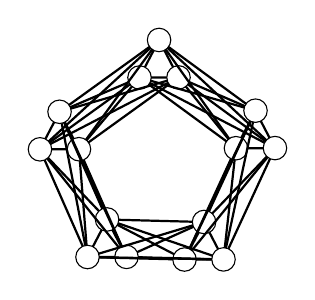
\begin{tikzpicture}[scale = 10]
\tikzstyle{VertexStyle}=[shape = circle, minimum size = 1pt, inner sep = 3pt,
draw]
\Vertex[x = 0.257401078939438, y = 0.729450404644012, L = \tiny {}]{v0}
\Vertex[x = 0.232565611600876, y = 0.681758105754852, L = \tiny {}]{v1}
\Vertex[x = 0.282104313373566, y = 0.681911885738373, L = \tiny {}]{v2}
\Vertex[x = 0.383801102638245, y = 0.820650428533554, L = \tiny {}]{v3}
\Vertex[x = 0.358965694904327, y = 0.772958129644394, L = \tiny {}]{v4}
\Vertex[x = 0.40850430727005, y = 0.773111909627914, L = \tiny {}]{v5}
\Vertex[x = 0.506290018558502, y = 0.730872631072998, L = \tiny {}]{v6}
\Vertex[x = 0.48145455121994, y = 0.683180332183838, L = \tiny {}]{v7}
\Vertex[x = 0.530993163585663, y = 0.683334112167358, L = \tiny {}]{v8}
\Vertex[x = 0.440956592559814, y = 0.589494824409485, L = \tiny {}]{v9}
\Vertex[x = 0.416121125221252, y = 0.541802525520325, L = \tiny {}]{v10}
\Vertex[x = 0.46565979719162, y = 0.541956305503845, L = \tiny {}]{v11}
\Vertex[x = 0.317756593227386, y = 0.592694818973541, L = \tiny {}]{v12}
\Vertex[x = 0.292921125888824, y = 0.545002520084381, L = \tiny {}]{v13}
\Vertex[x = 0.342459797859192, y = 0.545156300067902, L = \tiny {}]{v14}
\Edge[](v2)(v1)
\Edge[](v2)(v0)
\Edge[](v1)(v0)
\Edge[](v4)(v3)
\Edge[](v5)(v3)
\Edge[](v5)(v4)
\Edge[](v7)(v6)
\Edge[](v8)(v6)
\Edge[](v8)(v7)
\Edge[](v10)(v9)
\Edge[](v11)(v9)
\Edge[](v11)(v10)
\Edge[](v13)(v12)
\Edge[](v14)(v12)
\Edge[](v14)(v13)
\Edge[](v3)(v0)
\Edge[](v4)(v0)
\Edge[](v5)(v0)
\Edge[](v3)(v2)
\Edge[](v4)(v2)
\Edge[](v5)(v2)
\Edge[](v3)(v1)
\Edge[](v4)(v1)
\Edge[](v5)(v1)
\Edge[](v3)(v6)
\Edge[](v4)(v6)
\Edge[](v5)(v6)
\Edge[](v3)(v7)
\Edge[](v4)(v7)
\Edge[](v5)(v7)
\Edge[](v3)(v8)
\Edge[](v4)(v8)
\Edge[](v5)(v8)
\Edge[](v6)(v9)
\Edge[](v7)(v9)
\Edge[](v8)(v9)
\Edge[](v6)(v11)
\Edge[](v7)(v11)
\Edge[](v8)(v11)
\Edge[](v6)(v10)
\Edge[](v7)(v10)
\Edge[](v8)(v10)
\Edge[](v12)(v10)
\Edge[](v13)(v10)
\Edge[](v14)(v10)
\Edge[](v12)(v9)
\Edge[](v13)(v9)
\Edge[](v14)(v9)
\Edge[](v12)(v11)
\Edge[](v13)(v11)
\Edge[](v14)(v11)
\Edge[](v12)(v2)
\Edge[](v13)(v2)
\Edge[](v14)(v2)
\Edge[](v12)(v1)
\Edge[](v13)(v1)
\Edge[](v14)(v1)
\Edge[](v12)(v0)
\Edge[](v13)(v0)
\Edge[](v14)(v0)
\end{tikzpicture}}}}
\caption{Counterexamples to the Borodin-Kostochka Conjecture for small
$\Delta$.}
\label{fig:SmallCE}
\end{figure}



\bigskip
\noindent Known results:
\begin{itemize}
\item In 1980, Kostochka proved that if we exclude $K_{\Delta(G)-29}$ instead, then $G$ is $(\Delta(G)-1)$-colorable.
\item Later in the 1980s, Mozhan proved that if $\Delta(G) \geq 31$ and we exclude $K_{\Delta(G)-3}$ instead, then $G$ is $(\Delta(G)-1)$-colorable.
\item In 1999, Reed proved that the conjecture holds for $\Delta \geq 10^{14}$.  
\end{itemize}

\noindent Highlights:
\begin{itemize}
\item We prove the full Borodin-Kostochka conjecture for claw-free graphs.
\item We prove that the following conjecture is equivalent to the Borodin-Kostochka conjecture.
\begin{conjecture}
If $G$ is a graph with $\Delta(G) \geq 9$ such that $G$ doesn't contain $\join{K_3}{\overline{K}_{\Delta(G)-3}}$, then $G$ is $(\Delta(G)-1)$-colorable.
\end{conjecture}
\item We generalize Reed's result to list coloring:

\begin{thm}
There exists $\Delta_0$ such that every graph with $\Delta \geq \Delta_0$ that doesn't contain $K_{\Delta}$ is $(\Delta-1)$-choosable.
\end{thm}

Define $k$-choosable.
\end{itemize}

To illustrate the different proof ideas used i'm going to give a nonstandard proof of Brooks' theorem and then generalize parts of it.

\section{Brooks' theorem to illustrate parts}
\begin{thm}[Brooks 1941]
For $t \geq 3$, any graph with maximum degree at most $t$ that doesn't contain a $K_{t + 1}$ can be $t$-colored.
\end{thm}

\subsection{A proof}
\begin{enumerate}
\item Reduce to the cubic case.
\item Exclude diamonds.  PICTURE.
\item Exclude induced cycles.
\item Forests are bipartite.
\end{enumerate}

Suppose not and let $G$ be a counterexample with the minimum number of vertices.  By minimality of $\card{G}$, $G-v$ is $t$-colorable for each $v \in V(G)$.  In particular, $G$ is $t$-regular.

\textbf{Step (1).} \textit{Reduce to the cubic case}
Suppose $t \geq 4$. Consider a $t$-coloring of $G-v$ for some $v \in V(G)$.  Each color must be used on every $K_t$ in $G-v$ and hence some color must be used on every $K_t$ in $G$.  PICTURE.  

Let $M$ be such a color class expanded to a maximal independent set.  Then $\Delta(G-M) \leq t-1$ and $G-M$ contains no $K_t$, but $G-M$ cannot be $(t-1)$-colored, a contradiction.

\textbf{Step (2).} \textit{Exclude diamonds}
If $G$ has an induced diamond $D$, then after $3$-coloring $G-D$, we can color the nonadjacent vertices in $D$ the same and then finish greedily, impossible.  PICTURE.

\textbf{Step (3).} \textit{Exclude induced cycles}
Suppose $G$ contains an induced cycle $C$.   Since $K_4 \not \subseteq G$ we have $\card{N(C)} \geq 2$. PICTURE.

So, we may take different $x, y \in N(C)$ and put $H \DefinedAs G - C$ if $x$ is adjacent to $y$ and $H \DefinedAs (G-C) + xy$ otherwise.  PICTURE.

Then, $H$ doesn't contain $K_4$ as $G$ doesn't contain diamonds. PICTURE.

By minimality of $\card{G}$, $H$ is $3$-colorable. That is, we have a $3$-coloring of $G - C$ where $x$ and $y$ receive different colors, say $x$ gets $1$ and $y$ gets $2$.  Pick a neighbor $v_x$ in $C$ of $x$ and $v_y$ in $C$ of $y$.  Then $v_x$ has colors $2, 3$ available and $v_y$ has colors $1,3$ available.  PICTURE.

Follow a path from $v_x$ to $v_y$ to find adjacent vertices $p, q$ with different available color lists.  Color $p$ with a color $q$ doesn't have, then greedily color with $q$ last. PICTURE.

\textbf{Step (4).} \textit{Forests are bipartite.}
So, we're done.

\subsection{Generalizing pieces of the proof}
\subsubsection{Reducing maximum degree}
The reduction we just did worked by using the following idea.

Idea:  Find an independent set $I$ so that $\omega(G-I) < \omega(G)$.

\bigskip

Can such an $I$ can always be found?  No, take a $5$-cycle, PICTURE.  In fact, the graphs $G$ where for every induced subgraph $H$ of $G$ there exists $I$ such that $\omega(H-I) < \omega(H)$ are precisely the perfect graphs.  So, any odd hole or antihole provides an example.

\bigskip

But for our purposes we need less.  Suppose we could always find an $I$ when $\omega(G) \geq \Delta(G)$.  Then, if $\omega(G) \geq \Delta(G)$, expand the $I$ we get to a maximal independent set $M$, otherwise choose an arbitrary maximal independent set $M$.  Then we have $\omega(G-M) < \omega(G) \leq \Delta(G) - 1$ and $\Delta(G-M) \leq \Delta(G) - 1$,  hence $G-M$ is a smaller counterexample.

\bigskip

Let's look at the maximum cliques.  If $A$ and $B$ are maximum cliques that intersect, then $\card{A \cup B} \leq \Delta(G) + 1$, PICTURE. 

Thus $\card{A\cap B} = |A| + |B| - \card{A \cup B} \geq 2\omega(G) - (\Delta + 1) \geq \Delta(G) - 1 \geq 3$. Know: $G$ has no diamonds.  So, $A = B$. PICTURE.

\bigskip

PICTURE of clique blobs.  We just need to find an independent set with one vertex in each blob.  That is, we need to find an independent transversal.  First attempt might be to pick a vertex at random from each blob and apply the local lemma.  This only works for $\Delta \geq 6$.  In this simple case where each vertex has only one external neighbor, a simple algorithm will work (basic idea: pick a vertex, if it restricts a clique we haven't taken care of, pick a vertex in that clique, otherwise pick a vertex in some clique we haven't taken care of and repeat), but we want to generalize, so use:

\begin{lem}[Haxell]\label{HaxellLemma}
Let $H$ be a graph and $V_1 \cup \cdots \cup V_r$ a partition of $V(H)$. Suppose that $\card{V_i} \geq 2\Delta(H)$ for each $i \in \irange{r}$. Then $H$ has an independent set $\set{v_1, \ldots, v_n}$ where $v_i \in V_i$ for each $i \in \irange{r}$.
\end{lem}

The bound $2\Delta$ is best possible without further assumptions:

\begin{center}
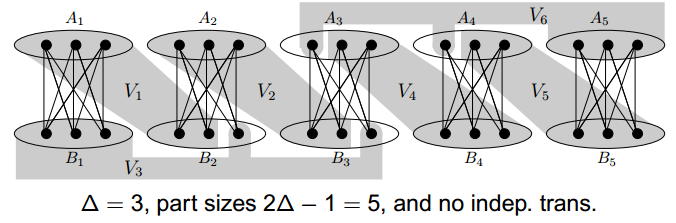
\includegraphics{notransversal.PNG}
\end{center}

This does the work for us and we have our desired independent set $I$ with $\omega(G-I) < \omega(G)$.

\bigskip\bigskip

Really, these reductions can be done with no conditions on the chromatic number. In 1980, Kostochka proved

\begin{lem}[Kostochka 1980]
If $G$ is a graph satisfying $\omega \geq \Delta + \frac32 - \sqrt{\Delta}$,
then $G$ contains an independent set $I$ such that $\omega(G - I) < \omega(G)$.
\end{lem}

In 2011, i improved the required condition to $\omega \geq \frac34 (\Delta + 1)$.  Finally, King improved the condition to $\omega > \frac23 (\Delta + 1)$, which is tight.  It follows from any of these results that the Borodin-Kostochka conjecture can be reduced to the $\Delta=9$ case.

\subsubsection{Excluding small subgraphs}
The argument used to exclude the diamond works in general: given any list assignment $L$ to the diamond where $\card{L(v)} \geq d(v)$, we can properly color from $L$.  A graph that has this property is called $d_0$-choosable and were classified in the 70s as follows.

\begin{ClassificationOfd0}
For any connected graph $G$, the following are equivalent.
\begin{itemize}
\item $G$ is $d_0$-choosable.
\item $G$ is not a Gallai tree.  DEFINITION and PICTURE.
\item $G$ contains an induced even cycle with at most one chord.
\end{itemize}
\end{ClassificationOfd0}

This generalizes Brooks' theorem since all regular Gallai trees with maximum degree at least $3$ are complete.

\bigskip\bigskip

Studying graphs that can be colored from any list assignment $L$ with $\card{L(v)} \geq d(v) - 1$ are similarly useful for $(\Delta(G) - 1)$-coloring graphs; these are the $d_1$-choosable graphs.   We didn't completely classify them, but we classified the $d_1$-choosable joins $\join{A}{B}$ where $\card{A}, \card{B} \geq 2$.
This was used to prove the full Borodin-Kostochka for claw-free graphs, I'll get back to that later.

\subsubsection{Adding edges to a subgraph}
In Step (3) of the proof of Brooks' theorem, we added an edge to $G-C$ to force two vertices to get different colors.  This trick is more generally useful.   Another useful trick we'll use is contracting an independent set. To use either of these we need to be in the context of a minimal counterexample.  It's cumbersome to carry this context around, so we're going to get rid of it by defining a strengthened notion of vertex critical graph.  We call these extra critical things \emph{mules}.

\begin{defn}
For any collection $\fancy{T}$ of graphs, a \emph{$\fancy{T}$-mule} is a $G \in \fancy{T}$ such that no homomorphic image of an induced subgraph of $G$ is in $\fancy{T}$ (besides $G$ itself).
\end{defn}

PICTURES.\bigskip

We're working with finite graphs, so $\fancy{T}$-mules exist for every nonempty $\fancy{T}$.  The identity homomorphism from a proper induced subgraph shows that this strengthens vertex critical. 

\bigskip

Let $\fancy{C}_k$ be the graphs $G$ with $\chi(G) \geq \Delta(G) = k$ and $\omega(G) < k$.  The Borodin-Kostochka conjecture says that $\fancy{C}_k$ is empty for $k \geq 9$. Using $\fancy{C}_k$-mules we get more information about small $k$ than we get from a minimum counterexample.  For example, these are both $\fancy{C}_7$-mules:

\begin{figure}[htb]
\centering
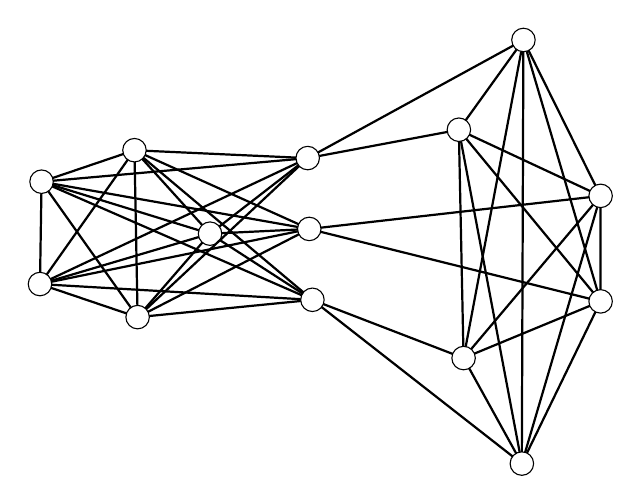
\begin{tikzpicture}[scale = 10]
\tikzstyle{VertexStyle}=[shape = circle,	
								 minimum size = 1pt,
								 inner sep = 3pt,
                         draw]
\Vertex[x = 0.751999914646149, y = 0.724000096321106, L = \tiny {}]{v0}
\Vertex[x = 0.751999974250793, y = 0.590000092983246, L = \tiny {}]{v1}
\Vertex[x = 0.652000069618225, y = 0.38400000333786, L = \tiny {}]{v2}
\Vertex[x = 0.578000009059906, y = 0.51800012588501, L = \tiny {}]{v3}
\Vertex[x = 0.572000086307526, y = 0.808000028133392, L = \tiny {}]{v4}
\Vertex[x = 0.0419999808073044, y = 0.742000013589859, L = \tiny {}]{v5}
\Vertex[x = 0.0399999916553497, y = 0.612000048160553, L = \tiny {}]{v6}
\Vertex[x = 0.163999989628792, y = 0.569999992847443, L = \tiny {}]{v7}
\Vertex[x = 0.25600004196167, y = 0.676000028848648, L = \tiny {}]{v8}
\Vertex[x = 0.159999996423721, y = 0.782000005245209, L = \tiny {}]{v9}
\Vertex[x = 0.653999924659729, y = 0.921999998390675, L = \tiny {}]{v10}
\Vertex[x = 0.379999995231628, y = 0.771999999880791, L = \tiny {}]{v11}
\Vertex[x = 0.381999999284744, y = 0.682000011205673, L = \tiny {}]{v12}
\Vertex[x = 0.386000007390976, y = 0.592000007629395, L = \tiny {}]{v13}
\Edge[](v0)(v4)
\Edge[](v1)(v4)
\Edge[](v2)(v4)
\Edge[](v3)(v4)
\Edge[](v0)(v3)
\Edge[](v1)(v3)
\Edge[](v2)(v3)
\Edge[](v0)(v2)
\Edge[](v1)(v2)
\Edge[](v0)(v1)
\Edge[](v5)(v6)
\Edge[](v5)(v7)
\Edge[](v5)(v8)
\Edge[](v5)(v9)
\Edge[](v6)(v7)
\Edge[](v6)(v8)
\Edge[](v6)(v9)
\Edge[](v7)(v8)
\Edge[](v7)(v9)
\Edge[](v8)(v9)
\Edge[](v0)(v10)
\Edge[](v1)(v10)
\Edge[](v2)(v10)
\Edge[](v3)(v10)
\Edge[](v4)(v10)
\Edge[](v5)(v11)
\Edge[](v6)(v11)
\Edge[](v7)(v11)
\Edge[](v8)(v11)
\Edge[](v9)(v11)
\Edge[](v5)(v12)
\Edge[](v6)(v12)
\Edge[](v7)(v12)
\Edge[](v8)(v12)
\Edge[](v9)(v12)
\Edge[](v5)(v13)
\Edge[](v6)(v13)
\Edge[](v7)(v13)
\Edge[](v8)(v13)
\Edge[](v9)(v13)
\Edge[](v11)(v10)
\Edge[](v11)(v4)
\Edge[](v12)(v0)
\Edge[](v12)(v1)
\Edge[](v13)(v3)
\Edge[](v13)(v2)
\end{tikzpicture}
\caption{The mule $M_{7,1}$.}
\label{fig:M_7}
\end{figure}

\begin{figure}[htb]
\centering
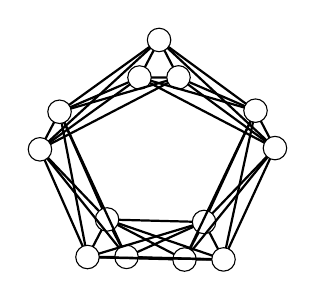
\begin{tikzpicture}[scale = 10]
\tikzstyle{VertexStyle}=[shape = circle,	
								 minimum size = 1pt,
								 inner sep = 3pt,
                         draw]
\Vertex[x = 0.257401078939438, y = 0.729450404644012, L = \tiny {}]{v0}
\Vertex[x = 0.232565611600876, y = 0.681758105754852, L = \tiny {}]{v1}
\Vertex[x = 0.383801102638245, y = 0.820650428533554, L = \tiny {}]{v2}
\Vertex[x = 0.358965694904327, y = 0.772958129644394, L = \tiny {}]{v3}
\Vertex[x = 0.40850430727005, y = 0.773111909627914, L = \tiny {}]{v4}
\Vertex[x = 0.506290018558502, y = 0.730872631072998, L = \tiny {}]{v5}
\Vertex[x = 0.530993163585663, y = 0.683334112167358, L = \tiny {}]{v6}
\Vertex[x = 0.440956592559814, y = 0.589494824409485, L = \tiny {}]{v7}
\Vertex[x = 0.416121125221252, y = 0.541802525520325, L = \tiny {}]{v8}
\Vertex[x = 0.46565979719162, y = 0.541956305503845, L = \tiny {}]{v9}
\Vertex[x = 0.317756593227386, y = 0.592694818973541, L = \tiny {}]{v10}
\Vertex[x = 0.292921125888824, y = 0.545002520084381, L = \tiny {}]{v11}
\Vertex[x = 0.342459797859192, y = 0.545156300067902, L = \tiny {}]{v12}
\Edge[](v1)(v0)
\Edge[](v3)(v2)
\Edge[](v4)(v2)
\Edge[](v4)(v3)
\Edge[](v6)(v5)
\Edge[](v8)(v7)
\Edge[](v9)(v7)
\Edge[](v9)(v8)
\Edge[](v11)(v10)
\Edge[](v12)(v10)
\Edge[](v12)(v11)
\Edge[](v2)(v0)
\Edge[](v3)(v0)
\Edge[](v4)(v0)
\Edge[](v2)(v1)
\Edge[](v3)(v1)
\Edge[](v4)(v1)
\Edge[](v2)(v5)
\Edge[](v3)(v5)
\Edge[](v4)(v5)
\Edge[](v2)(v6)
\Edge[](v3)(v6)
\Edge[](v4)(v6)
\Edge[](v5)(v7)
\Edge[](v6)(v7)
\Edge[](v5)(v9)
\Edge[](v6)(v9)
\Edge[](v5)(v8)
\Edge[](v6)(v8)
\Edge[](v10)(v8)
\Edge[](v11)(v8)
\Edge[](v12)(v8)
\Edge[](v10)(v7)
\Edge[](v11)(v7)
\Edge[](v12)(v7)
\Edge[](v10)(v9)
\Edge[](v11)(v9)
\Edge[](v12)(v9)
\Edge[](v10)(v1)
\Edge[](v11)(v1)
\Edge[](v12)(v1)
\Edge[](v10)(v0)
\Edge[](v11)(v0)
\Edge[](v12)(v0)
\end{tikzpicture}
\caption{The mule $M_{7,2}$.}
\label{fig:M_72}
\end{figure}



The first one has $14$ vertices while the second has $15$. Both are constructed by our proofs, but since the second one has more vertices it would not be constructed by a minimum counterexample argument.

\bigskip

The main result we proved about mules is

\begin{lem}\label{K3sOut}
For $k \geq 7$, the only $\fancy{C}_k$-mules containing $\join{K_3}{\overline{K}_{k-3}}$
as a subgraph are $M_{7,1}$,  $M_{7,2}$ and $M_8$.
\end{lem}

Here $M_8$ is the only known (connected) counterexample with $\Delta=8$.

\begin{figure}[htb]
\centering
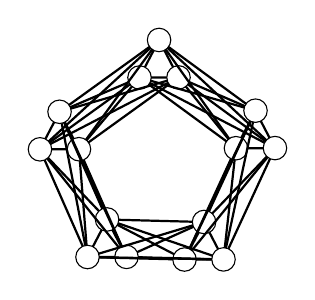
\begin{tikzpicture}[scale = 10]
\tikzstyle{VertexStyle}=[shape = circle,	
								 minimum size = 1pt,
								 inner sep = 3pt,
                         draw]
\Vertex[x = 0.257401078939438, y = 0.729450404644012, L = \tiny {}]{v0}
\Vertex[x = 0.232565611600876, y = 0.681758105754852, L = \tiny {}]{v1}
\Vertex[x = 0.282104313373566, y = 0.681911885738373, L = \tiny {}]{v2}
\Vertex[x = 0.383801102638245, y = 0.820650428533554, L = \tiny {}]{v3}
\Vertex[x = 0.358965694904327, y = 0.772958129644394, L = \tiny {}]{v4}
\Vertex[x = 0.40850430727005, y = 0.773111909627914, L = \tiny {}]{v5}
\Vertex[x = 0.506290018558502, y = 0.730872631072998, L = \tiny {}]{v6}
\Vertex[x = 0.48145455121994, y = 0.683180332183838, L = \tiny {}]{v7}
\Vertex[x = 0.530993163585663, y = 0.683334112167358, L = \tiny {}]{v8}
\Vertex[x = 0.440956592559814, y = 0.589494824409485, L = \tiny {}]{v9}
\Vertex[x = 0.416121125221252, y = 0.541802525520325, L = \tiny {}]{v10}
\Vertex[x = 0.46565979719162, y = 0.541956305503845, L = \tiny {}]{v11}
\Vertex[x = 0.317756593227386, y = 0.592694818973541, L = \tiny {}]{v12}
\Vertex[x = 0.292921125888824, y = 0.545002520084381, L = \tiny {}]{v13}
\Vertex[x = 0.342459797859192, y = 0.545156300067902, L = \tiny {}]{v14}
\Edge[](v2)(v1)
\Edge[](v2)(v0)
\Edge[](v1)(v0)
\Edge[](v4)(v3)
\Edge[](v5)(v3)
\Edge[](v5)(v4)
\Edge[](v7)(v6)
\Edge[](v8)(v6)
\Edge[](v8)(v7)
\Edge[](v10)(v9)
\Edge[](v11)(v9)
\Edge[](v11)(v10)
\Edge[](v13)(v12)
\Edge[](v14)(v12)
\Edge[](v14)(v13)
\Edge[](v3)(v0)
\Edge[](v4)(v0)
\Edge[](v5)(v0)
\Edge[](v3)(v2)
\Edge[](v4)(v2)
\Edge[](v5)(v2)
\Edge[](v3)(v1)
\Edge[](v4)(v1)
\Edge[](v5)(v1)
\Edge[](v3)(v6)
\Edge[](v4)(v6)
\Edge[](v5)(v6)
\Edge[](v3)(v7)
\Edge[](v4)(v7)
\Edge[](v5)(v7)
\Edge[](v3)(v8)
\Edge[](v4)(v8)
\Edge[](v5)(v8)
\Edge[](v6)(v9)
\Edge[](v7)(v9)
\Edge[](v8)(v9)
\Edge[](v6)(v11)
\Edge[](v7)(v11)
\Edge[](v8)(v11)
\Edge[](v6)(v10)
\Edge[](v7)(v10)
\Edge[](v8)(v10)
\Edge[](v12)(v10)
\Edge[](v13)(v10)
\Edge[](v14)(v10)
\Edge[](v12)(v9)
\Edge[](v13)(v9)
\Edge[](v14)(v9)
\Edge[](v12)(v11)
\Edge[](v13)(v11)
\Edge[](v14)(v11)
\Edge[](v12)(v2)
\Edge[](v13)(v2)
\Edge[](v14)(v2)
\Edge[](v12)(v1)
\Edge[](v13)(v1)
\Edge[](v14)(v1)
\Edge[](v12)(v0)
\Edge[](v13)(v0)
\Edge[](v14)(v0)
\end{tikzpicture}
\caption{$M_8$: A $C_5$ with vertices blown-up to triangles.}
\label{fig:M_8}
\end{figure}


Since $\join{K_3}{\overline{K}_{\Delta-3}} \subseteq K_\Delta$, Lemma \ref{K3sOut} shows
that Conjecture \ref{K3Conjecture} is equivalent to the Borodin-Kostochka
conjecture.

\begin{conjecture}\label{K3Conjecture}
If $G$ is a graph with $\Delta(G) \geq 9$ such that $G$ doesn't contain $\join{K_3}{\overline{K}_{\Delta(G)-3}}$, then $G$ is $(\Delta(G)-1)$-colorable.
\end{conjecture}

\section{Borodin-Kostochka for claw-free graphs}
Reminder $d_1$-choosable definition. We classified the $d_1$-choosable graph joins $\join{A}{B}$ where $\card{A}, \card{B} \geq 2$, this gives a lot more structure about a counterexample.  The classification takes 45 pages to prove, we won't go into it, but will use the results to prove Borodin-Kostochka for claw-free graphs.

\bigskip
We outline the proof of the following.
\begin{thm}
Every claw-free graph with $\Delta \geq 9$ that doesn't contain $K_{\Delta}$ can be $(\Delta-1)$-colored.
\end{thm}

The proof uses the structure theorem for claw-free graphs proved by Chudnovsky and Seymour. We actually only need a simpler part of it: the structure theorem for quasi-line graphs; graphs where the neighborhood of every vertex can be covered by two cliques.  PICTURE.

\bigskip

We use the following structure theorem for quasi-line graphs.

\begin{lem}\label{QuasilineStructure}
Every connected skeletal quasi-line graph is a circular interval graph or a composition of
linear interval strips.
\end{lem}

We need to define the terms in this lemma.

A \emph{homogeneous pair of cliques} $(A_1, A_2)$ in a graph $G$ is a pair of
disjoint nonempty cliques such that for each $i \in \irange{2}$, every vertex in
$G - (A_1 \cup A_2)$ is either joined to $A_i$ or misses all of $A_i$ and
$\card{A_1} + \card{A_2} \geq 3$. PICTURES.

A homogeneous pair of cliques $(A_1, A_2)$ is $\emph{skeletal}$
if for any $e \in E(A, B)$ we have $\omega(G[A \cup B] - e) < \omega(G[A \cup
B])$.  A graph is $\emph{skeletal}$ if it contains no nonskeletal homogeneous
pair of cliques.  

\bigskip

Given a set $V$ of points on the unit circle together with a set of closed intervals $C$ on the unit circle we define a graph with vertex set $V$ and an edge between two different vertices if and only if they are both contained in some element of $C$.  Any graph isomorphic to such a graph is a \emph{circular interval graph}.  Similarly, by replacing the unit circle with the unit interval, we get the class of \emph{linear interval graphs}.

\bigskip

It remains to define \emph{compositions of linear interval strips}.  These are a generalization of line graphs. 
A \emph{linear interval strip} $(S, A_1, A_2)$ is a linear interval graph $S$ together with end cliques $A_1$ and $A_2$.  PICTURE.

\bigskip

Let $H$ be a directed multigraph (possibly with loops)
and suppose for each edge $e$ of $H$ we have a strip $(S_e, X_e, Y_e)$.  For
each $v \in V(H)$ define

\[C_v \DefinedAs \parens{\bigcup \setbs{X_e}{\text{$e$ is directed out of $v$}}}
\cup \parens{\bigcup \setbs{Y_e}{\text{$e$ is directed into $v$}}}\]

The graph formed by taking the disjoint union of $\setbs{S_e}{e \in E(H)}$ and
making $C_v$ a clique for each $v \in V(H)$ is the composition of the strips
$(S_e, X_e, Y_e)$.  Any graph formed in such a manner is called a
\emph{composition of linear interval strips}.  PICTURE.

Taking all strips to have a single vertex gives the line graph construction.

\bigskip\bigskip

Now we can outline the proof.

\begin{enumerate}
\item Prove for circular interval graphs.
\item Reduce from quasi-line graphs to line graphs as follows:
	\begin{enumerate}
	\item It is always possible to make skeletal counterexample from a given counterexample just by removing edges in nonskeletal homogeneous pairs of cliques.  Do so.
	\item We must have a composition of linear interval strips by the structure theorem.
	\item Take a composition representation using the maximum number of strips.
	\item Show that for each strip $(S, A_1, A_2)$ we must have $V(S) = A_1 = A_2$ and thus we have a line graph.
	\end{enumerate}
\item Prove for line graphs of multigraphs.
\item Reduce from claw-free graphs to quasi-line graphs.
\end{enumerate}

Steps (1), (2) and (4) all rely heavily on our classification of $d_1$-choosable joins.  Step (4) uses some $d_1$-choosability results outside this classification, for example, the following graph $D_8$ is $d_1$-choosable:

\begin{figure}[htb]
\centering
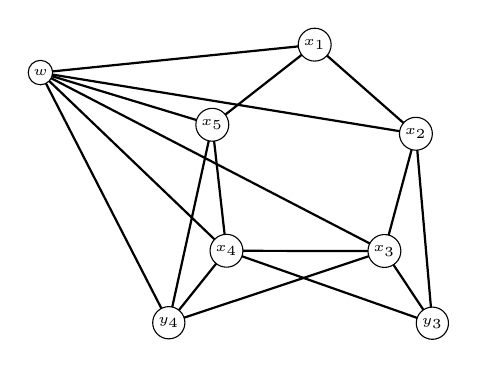
\begin{tikzpicture}[scale = 10]
\tikzstyle{VertexStyle}=[shape = circle,	
								 minimum size = 1pt,
								 inner sep = 1.2pt,
                         draw]
\Vertex[x = 0.535568237304688, y = 0.836275801062584, L = \tiny {$x_2$}]{v0}
\Vertex[x = 0.294997036457062, y = 0.687704384326935, L = \tiny {$x_4$}]{v1}
\Vertex[x = 0.495568662881851, y = 0.687386810779572, L = \tiny {$x_3$}]{v2}
\Vertex[x = 0.276996433734894, y = 0.847704276442528, L = \tiny {$x_5$}]{v3}
\Vertex[x = 0.556489169597626, y = 0.595672339200974, L = \tiny {$y_3$}]{v4}
\Vertex[x = 0.0587111786007881, y = 0.913989931344986, L = \tiny {$w$}]{v5}
\Vertex[x = 0.221746027469635, y = 0.596272975206375, L = \tiny {$y_4$}]{v6}
\Vertex[x = 0.407015770673752, y = 0.949415870010853, L = \tiny {$x_1$}]{v7}
\Edge[](v2)(v0)
\Edge[](v2)(v1)
\Edge[](v3)(v1)
\Edge[](v4)(v1)
\Edge[](v0)(v5)
\Edge[](v1)(v5)
\Edge[](v2)(v5)
\Edge[](v3)(v5)
\Edge[](v4)(v2)
\Edge[](v4)(v0)
\Edge[](v6)(v1)
\Edge[](v6)(v5)
\Edge[](v6)(v3)
\Edge[](v6)(v2)
\Edge[](v7)(v3)
\Edge[](v7)(v0)
\Edge[](v7)(v5)
\end{tikzpicture}
\caption{The graph $D_8$.}
\label{fig:D8}
\end{figure}


The reduction from claw-free graphs to quasi-line graphs works for list coloring as well.  Also, the circular interval graphs proof works for list coloring.  So, the following generalization seems within reach.

\begin{conjecture}
Every claw-free graph with $\Delta \geq 9$ that doesn't contain $K_{\Delta}$ is $(\Delta-1)$-choosable.
\end{conjecture}

Borodin and Kostochka conjecture that this holds with the claw-free restriction removed.  As evidence of this, we generalized Reed's proof of Borodin-Kostochka for large $\Delta$ to list coloring, proving:

\begin{thm}
There exists $\Delta_0$ such that every graph with $\Delta \geq \Delta_0$ that doesn't contain $K_{\Delta}$ is $(\Delta-1)$-choosable.
\end{thm}

\section{Future directions}
\begin{enumerate}
\item BK for list coloring for claw-free graphs.
\item improved bounds on the number of edges in (online) list-critical.  These can be used to prove Ore degree bounds for (online) list coloring; we have so far that the Ore degree version of Brooks' theorem for (online) list coloring holds for $\Delta \geq 11$.
\item Improve Mozhan's methods to get down to $\Delta-2$, we can now prove his $\Delta-3$ result for $\Delta \geq 13$ instead of $\Delta \geq 31$, and the proof is relatively simple.
\item BK for large $\Delta$ for online list coloring (and Alon-Tarsi number)
\end{enumerate}
\end{document}
